% !TEX root = ../../../main.tex
% 来源：中学数学实验教材·第三册（高中数学）
% 章节：函数及其图象 / 函数及其图象
% 原始文件：4.tex，行 928-946
% 类型：tikz
% ---
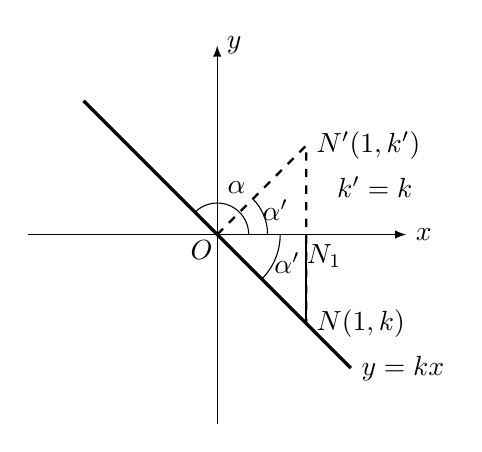
\begin{tikzpicture}[>=latex, scale=.8]
    \draw[->](-3,0)--(3,0)node[right]{$x$};
    \draw[->] (0,-3)--(0,3)node[right]{$y$};
    \node at (-.25,-.25){$O$};
    \draw[very thick] (0,0)--(-45:3)node[right]{$y=kx$};
    \draw[very thick] (0,0)--(135:3);
\draw [dashed, thick](0,0)--(45:2)node[right]{$N'(1,k')$}--(-45:2);
\draw[thick](1.414,0)--(1.414,-1.414)node[right]{$N(1,k)$};
\node at (1.7,0) [below]{$N_1$};
\node at (2.5,.75){$k'=k$};
\draw (.5,0) arc (0:135:.5);
\draw (.8,0) arc (0:45:.8);
\draw (1,0) arc (0:-45:1);

\node at (22.5:1){$\alpha'$};
\node at (-22.5:1.2){$\alpha'$};
\node at (67.5:.8){$\alpha$};

\end{tikzpicture}
